% Created 2020-04-13 Mon 21:14
% Intended LaTeX compiler: pdflatex
\documentclass[11pt]{article}
\usepackage[utf8]{inputenc}
\usepackage[T1]{fontenc}
\usepackage{graphicx}
\usepackage{grffile}
\usepackage{longtable}
\usepackage{wrapfig}
\usepackage{rotating}
\usepackage[normalem]{ulem}
\usepackage{amsmath}
\usepackage{textcomp}
\usepackage{amssymb}
\usepackage{capt-of}
\usepackage{hyperref}
\author{Dustin Leatherman}
\date{\today}
\title{Homework 2}
\hypersetup{
 pdfauthor={Dustin Leatherman},
 pdftitle={Homework 2},
 pdfkeywords={},
 pdfsubject={},
 pdfcreator={Emacs 26.3 (Org mode 9.4)}, 
 pdflang={English}}
\begin{document}

\maketitle
\tableofcontents


\section{Problem Statement}
\label{sec:org2d4f75c}

Find the point on the sphere \(x^2 + y^2 + z^2 = 9\) that are closest to and
farthest away from the point (2,3,4).


Hint: Construct and use a Jacobian Matrix. i.e gradient vector(s)

\section{Solution}
\label{sec:orgcfc2023}

Let the function to be minimized be represented as
$$
f(x,y,z) = (x - 2)^2 + (y - 3)^2 + (z - 4)^2 = d^2
$$

where \(d^2\) is distance squared. \(f(x,y,z)\) represents the distance squared between (x,y,z) and
(2,3,4).

Let the constraint function be represented as
$$
g(x,y,z) = x^2 + y^2 + z^2 = 9
$$

The Jacobian Matrix is a matrix of partial derivatives with \(N = 3\) columns and
\(m = 1\) rows. Let the Jacobian matrix for \(f(x,y,z)\) be described as
$$
\nabla f(x,y,z) = \begin{bmatrix}
\frac{\partial f(x,y,z)}{\partial x} & \frac{\partial f(x,y,z)}{\partial y} &
\frac{\partial f(x,y,z)}{\partial z}
\end{bmatrix} = \begin{bmatrix}
2(x - 2) & 2(y - 3) & 2(z - 4)
\end{bmatrix}
$$

and the Jacobian Matrix for \(g(x,y,z)\) be

$$
\nabla g(x,y,z) = \begin{bmatrix}
\frac{\partial g(x,y,z)}{\partial x} & \frac{\partial g(x,y,z)}{\partial y} &
\frac{\partial g(x,y,z)}{\partial z}
\end{bmatrix} = \begin{bmatrix}
2x & 2y & 2z
\end{bmatrix}
$$

at the closest value for \(g(x,y,z) = 9\).

\begin{figure}[htbp]
\centering
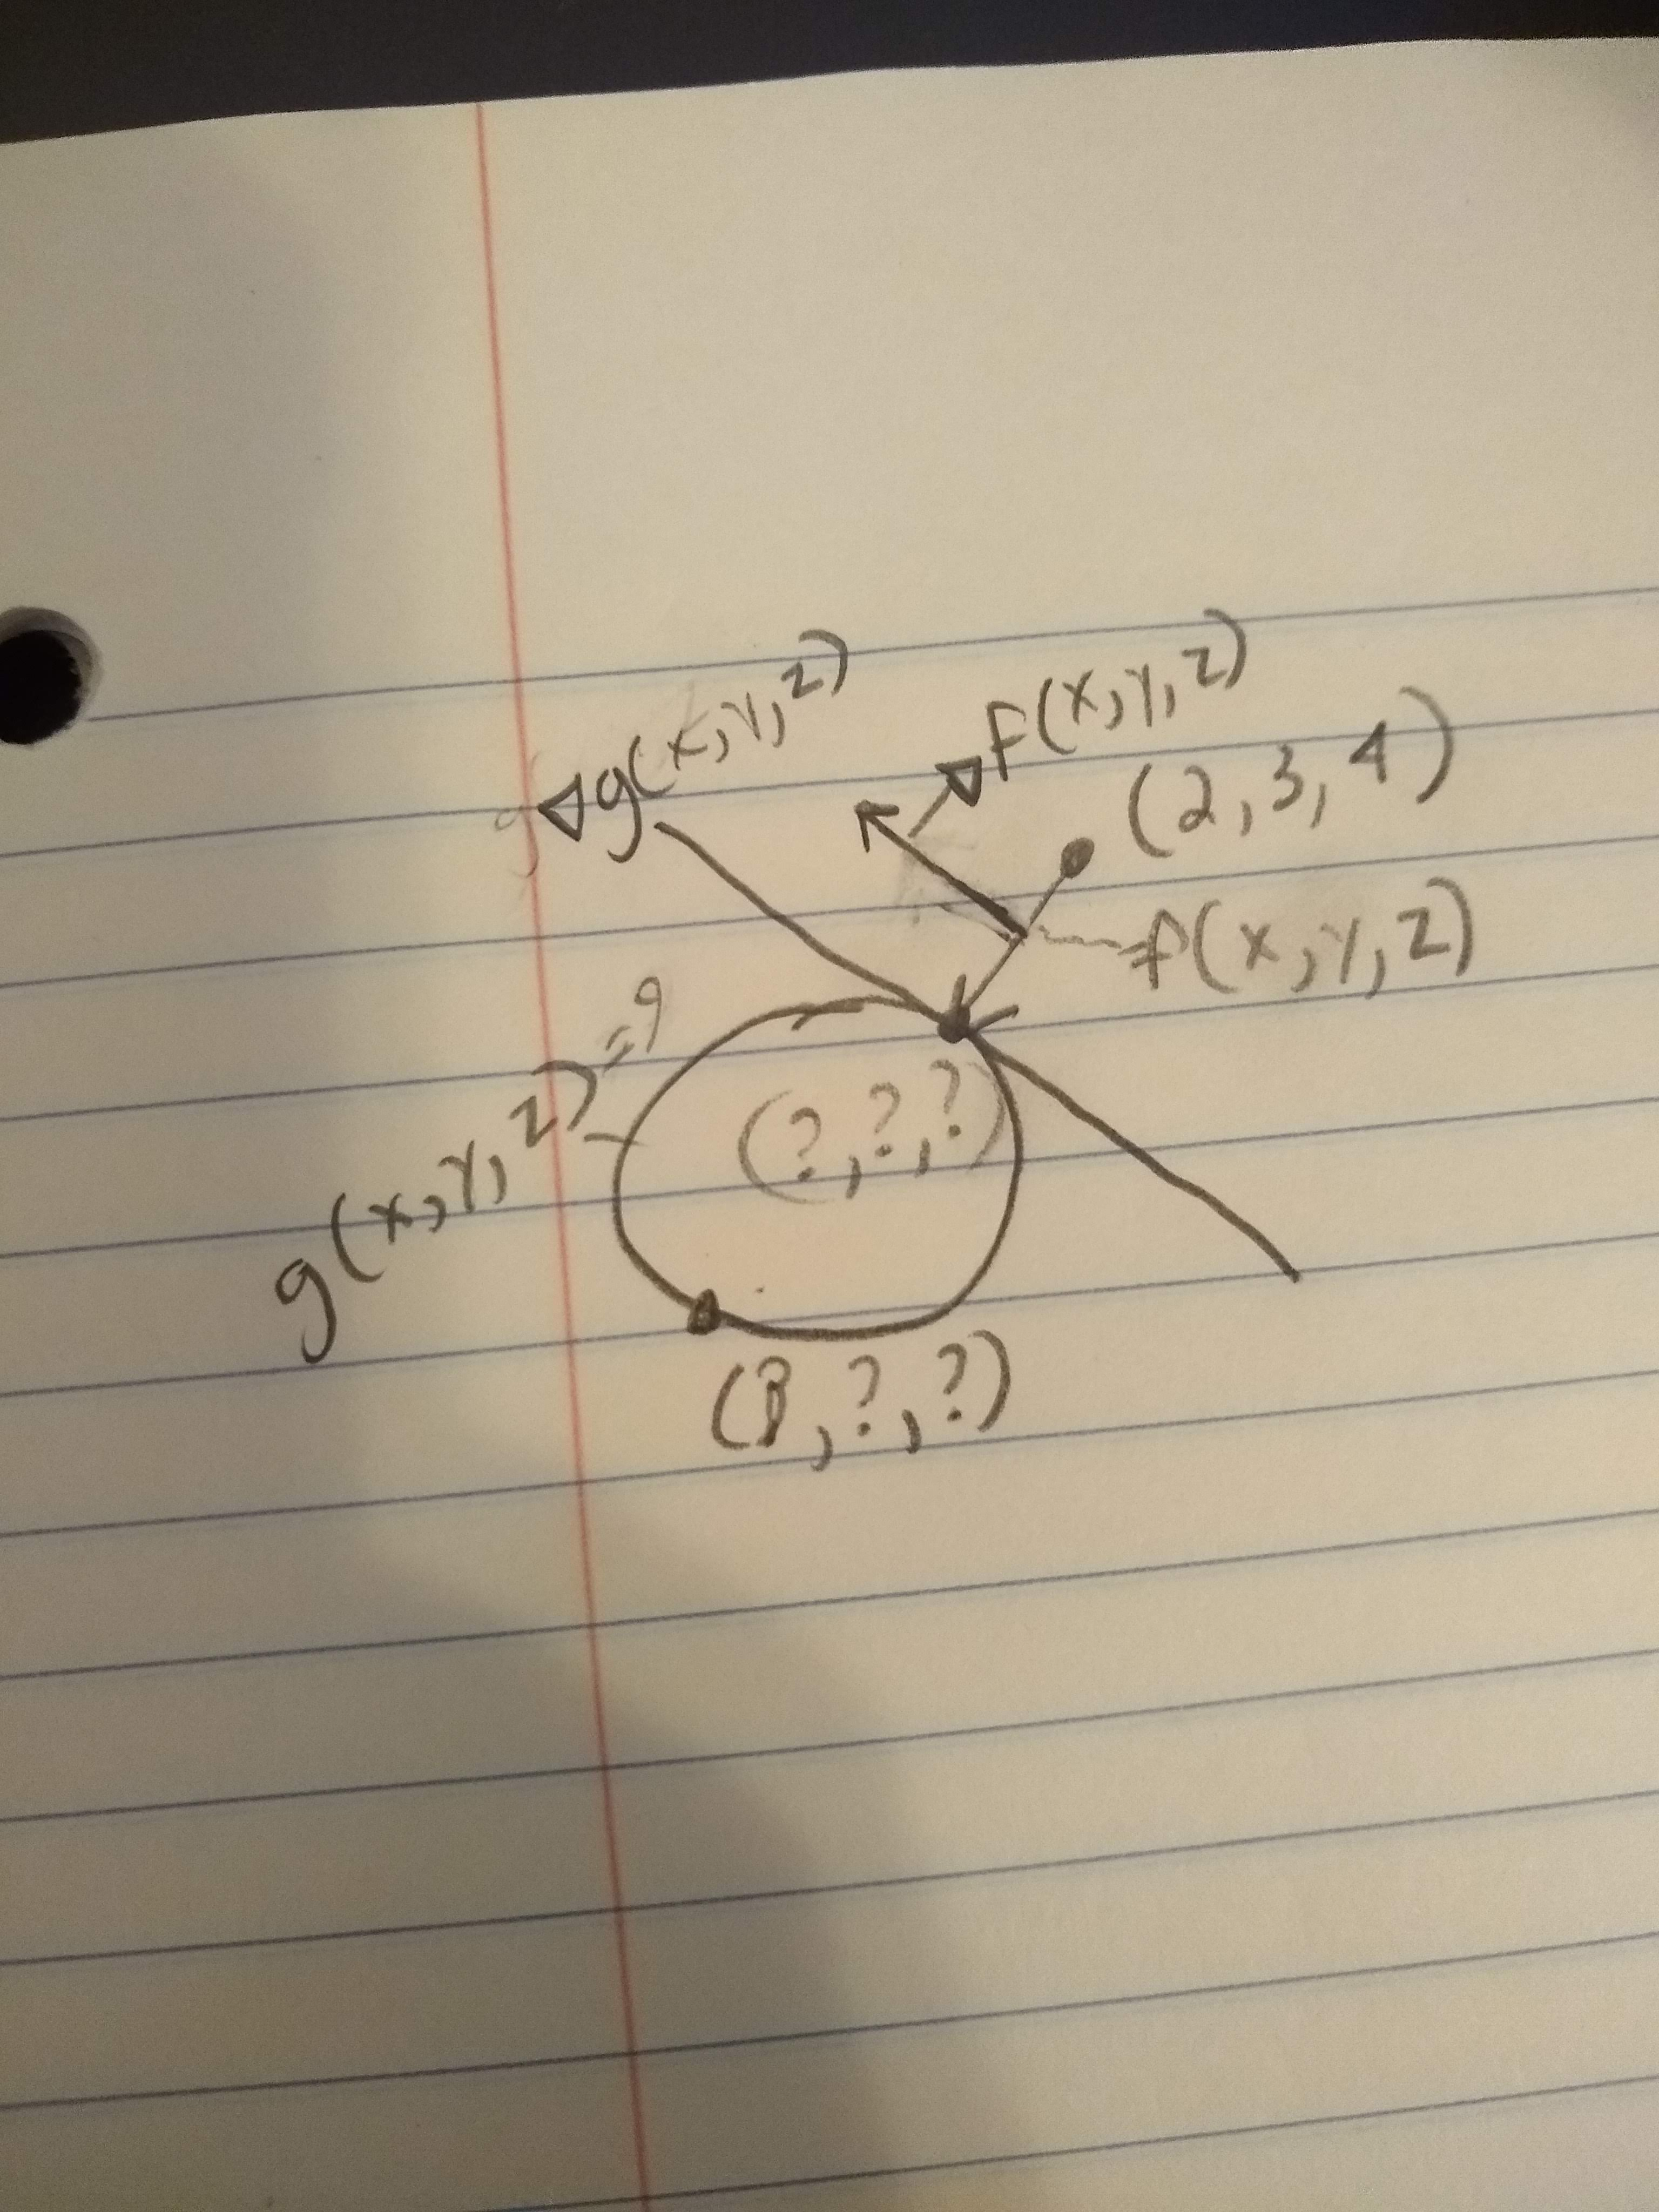
\includegraphics[width=10.6cm,height=7cm\textwidth]{./resources/homework2.jpg}
\caption{\label{fig:org96ae625}2-D sketch of the problem}
\end{figure}


Since a function and its gradient vector are perpendicular, it can be shown that
\(\nabla f\) and \(\nabla g\) are parallel. Thus it can be said, \(\nabla f = \lambda
\ \nabla g\) where \(\lambda\) is some constant.

This can be represented by the system of equations

\begin{subequations}
\label{first:main}
\begin{align}
2(x - 2) = & 2x \lambda \label{first:a}\\
2(y - 3) = & 2y \lambda \label{first:b} \\
2(z - 4) = & 2z \lambda \label{first:c} \\
x^2 + y^2 + z^2 = & 9 \label{first:d}
\end{align}
\end{subequations}

Solving \(\eqref{first:a} - \eqref{first:c}\) in terms of \(\lambda\) will then be
plugged into \(\eqref{first:d}\) to determine the points on \(g(x,y,z) = 9\) closest
and furthest from (2,3,4).

\textbf{1a}

\begin{equation}
\begin{split}
2(x - 2) = & 2 x \lambda\\
x - 2 = & x \lambda\\
\frac{2}{1 - \lambda} = &  x
\end{split}
\end{equation}

\textbf{1b}

\begin{equation}
\begin{split}
2(y - 3) = & 2 y \lambda\\
y - 3 = & y \lambda\\
\frac{3}{1 - \lambda} = & y
\end{split}
\end{equation}

\textbf{1c}

\begin{equation}
\begin{split}
2(z - 4) = & 2 z \lambda\\
z - 4 = & z \lambda\\
\frac{4}{1 - \lambda} = & z
\end{split}
\end{equation}

\textbf{1d}

\begin{equation}
\begin{split}
(\frac{2}{1 - \lambda})^2 + (\frac{3}{1 - \lambda})^2 + (\frac{4}{1 - \lambda})^2 = & 9\\
\frac{4}{(1 - \lambda)^2} + \frac{9}{(1 - \lambda)^2} + \frac{16}{(1 - \lambda)^2} = & 9\\
\frac{29}{(1 - \lambda)^2} = & 9\\
(1 - \lambda)^2 = & \frac{29}{9}\\
1 - \lambda = \frac{\sqrt{29}}{3} \ \text{OR} \ & 1 - \lambda = - \frac{\sqrt{29}}{3}\\
1 \pm \frac{\sqrt{29}}{3} = & \lambda
\end{split}
\end{equation}

For (2,3,4) and \(\lambda = 1 - \frac{\sqrt{29}}{3}\),

\begin{equation}
\begin{split}
\frac{2}{1 - \lambda} = & x\\
\frac{2}{1 - (1 + \frac{\sqrt{29}}{3})} = & x\\
\frac{-6}{\sqrt{29}} = & x
\end{split}
\end{equation}

\begin{equation}
\begin{split}
\frac{2}{1 - \lambda} = & x\\
\frac{2}{1 - (1 - \frac{\sqrt{29}}{3})} = & x\\
\frac{6}{\sqrt{29}} = & x
\end{split}
\end{equation}


\begin{equation}
\begin{split}
\frac{3}{1 - \lambda} = & y\\
\frac{3}{1 - (1 + \frac{\sqrt{29}}{3})} = & y\\
\frac{-9}{\sqrt{29}} = & y
\end{split}
\end{equation}

\begin{equation}
\begin{split}
\frac{3}{1 - \lambda} = & y\\
\frac{3}{1 - (1 - \frac{\sqrt{29}}{3})} = & y\\
\frac{9}{\sqrt{29}} = & y
\end{split}
\end{equation}


\begin{equation}
\begin{split}
\frac{4}{1 - \lambda} = & z\\
\frac{4}{1 - (1 + \frac{\sqrt{29}}{3})} = & z\\
\frac{-12}{\sqrt{29}} = & z
\end{split}
\end{equation}

\begin{equation}
\begin{split}
\frac{4}{1 - \lambda} = & z\\
\frac{4}{1 - (1 - \frac{\sqrt{29}}{3})} = & z\\
\frac{12}{\sqrt{29}} = & z
\end{split}
\end{equation}

Let P be the point when \(\lambda = 1 - \frac{\sqrt{29}}{3}\), then  \(P(\frac{6}{\sqrt{29}}, \frac{9}{\sqrt{29}}, \frac{12}{\sqrt{29}}))\)

Let Q be the point when \(\lambda = 1 + \frac{\sqrt{29}}{3}\), then \(Q(\frac{-6}{\sqrt{29}}, \frac{-9}{\sqrt{29}}, \frac{-12}{\sqrt{29}}))\)

Since all values for P are positive and all values of Q are negative, it follows that P is the closest point to (2,3,4) on the sphere
\(x^2 + y^2 + z^2 = 9\) and Q is the furthest.
\end{document}
